\documentclass[a4paper]{scrartcl}

\usepackage{amsmath}
\usepackage{amsfonts}
\usepackage{xcolor}
\usepackage{graphicx}
\usepackage{listings}
\usepackage{float}
\usepackage{hyperref}


\newcommand{\elbo}{\mathcal{L}}
\newcommand{\E}{\mathbb{E}}
\newcommand{\p}{\mathbb{P}}



\title{Pre Study}
\subtitle{Literature review}
\author{
Bruno Carchia \\
\texttt{carchia@kth.se}
}

\begin{document}
\maketitle
\section{Introduction}
This section provides a critical analysis of the literature and technical reports that informed the selection of the methodologies and technologies employed in this research. Each reviewed paper contributed specifically to the architectural design or the strategic formulation of the Reinforcement Learning agent. To ensure clarity, each work is presented using the following structure:

\begin{itemize}
    \item \textbf{Core Summary:} A brief overview of the research objectives and findings of the paper.
    \item \textbf{Technical Contribution:} An explanation of how the paper's insights directly influenced the development of this thesis.
\end{itemize}


\section{An advanced learning environment and a scalable deep reinforcement learning approach for rolling stock circulation on urban rail transit line}
This study \cite{YANG2025104976} addresses the Rolling Stock Circulation (RSC) problem by formulating it as a multi-objective optimization task within a Deep Reinforcement Learning framework. The primary objectives identified are the minimization of fleet utilization, the balancing of maintenance workloads, and the stabilization of depot stock levels. 

\textbf{State Space Representation} \\
The authors define a hierarchical state representation where the global state $s^t$ is a concatenation of individual rolling stock statuses $s_k^t$. The local state for each asset $k$ is defined as a six-dimensional feature vector:
$$
s_k^t = \left(n_k^t, \bar{c}_k^t, \bar{b}_k^t, f_k^t, o_k^t, g_k^t \right)
$$
This vector captures critical operational constraints, including cumulative trip counts ($n_k^t$), remaining service life ($\bar{c}_k^t$), and turnaround readiness ($f_k^t$). Notably, the inclusion of operation direction ($o_k^t$) and a timetable pointer ($g_k^t$) ensures the agent maintains the Markov property by encoding the physical feasibility of future assignments.

\textbf{Action Space} \\
The action space $A = \{1, 2, \dots, |K|\}$ is discrete, where each action corresponds to the selection of a specific physical asset from the fleet. To handle the "hard constraints" of rail operations (e.g., assigning a busy train), the authors utilize a penalty-based approach rather than strict action masking. This forces the agent to learn the underlying feasibility logic through the negative reinforcement of invalid selections.

\textbf{Reward Mechanism} \\
A dual-reward structure is employed to handle the credit assignment problem:
\begin{enumerate}
    \item \textbf{Dense Step-wise Reward ($r'$):} Focused on immediate utilization efficiency and constraint satisfaction. It penalizes unnecessary depot extractions ($r_a$) and rewards the selection of idle assets with high turnaround times ($r_v$), promoting a "First-In, First-Out" logic.
    \item \textbf{Sparse Terminal Reward ($Z$):} A weighted sum of normalized objectives calculated at the end of the operation horizon. This term targets fleet-wide fairness (workload standard deviation $z_3$) and depot equilibrium ($z_2$).
\end{enumerate}
\begin{figure}[H]
    \centering
    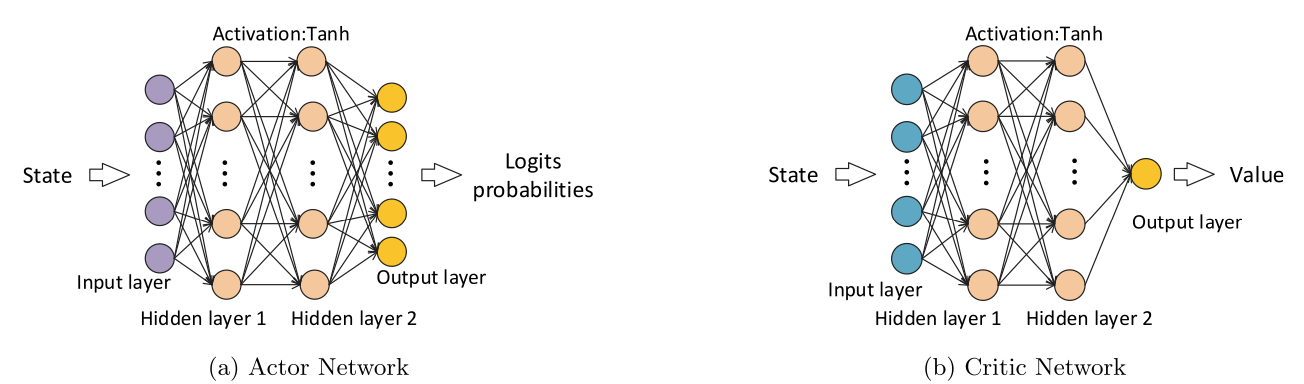
\includegraphics[width=\textwidth]{../images/pre_study/ActorCriticNetworkArchitecture.png}
    \caption{Architecture of the proposed Actor-Critic Neural Network. Taken from (Yang et al., 2025 \cite{YANG2025104976}) }
    \label{fig:ac_architecture}
\end{figure}
\textbf{Neural Network Architecture} \\
The problem is solved using the Proximal Policy Optimization (PPO) algorithm. As illustrated in Figure \ref{fig:ac_architecture}, the Actor and Critic networks utilize a fully-connected Multi-Layer Perceptron (MLP) structure with hyperbolic tangent ($\tanh$) activation functions. 

\textbf{Technical Contribution and Relevance to Thesis} \\
This paper provides the foundational logic for my research, particularly in the structuring of sparse and dense rewards to balance local efficiency with global maintenance goals. However, while the authors utilize a global MLP that scales linearly with fleet size, my work improves upon this by implementing a \textbf{Shared-Weight MLP}. This ensures that the model is permutation-invariant and can generalize to varying fleet sizes without re-training—a significant limitation observed in the original paper's architecture.

\begin{table}[H]
    \centering
    % Adjusting column widths: p{3cm} for features, p{5cm} for the others
    \begin{tabular}{|p{3.5cm}|p{5cm}|p{5.5cm}|}
        \hline
        \textbf{Feature} & \textbf{Reference Paper} & \textbf{This Thesis} \\ \hline
        \textbf{Algorithm} & PPO (Actor-Critic) & PPO (Actor-Critic) \\ \hline
        \textbf{Action Space} & Discrete (Fixed $|K|$) & Continuous Weights (Scalable) \\ \hline
        \textbf{NN Architecture} & Global Flat MLP & Shared-Weight Architecture \\ \hline
        \textbf{Observation Space} & Fixed Global Vector & Masked Relational Features \\ \hline
        \textbf{Maintenance Logic} & Reactive (Fixed Thresholds) & Proactive (Weibull-based) \\ \hline
        \textbf{Simulation Type} & Step-based & Event-driven \\ \hline
    \end{tabular}
    \caption{Comparative analysis between the reference study and the proposed DRL approach.}
    \label{tab:methodology_comparison}
\end{table}

\section{Deep Reinforcement Learning for Integrated Train Scheduling and Rolling Stock Circulation}

A significant contribution to integrated rail optimization is presented by Zhao et al. \cite{ZHAO2026111784}, who propose a Deep Reinforcement Learning (DRL) approach to solve the joint problem of train scheduling and rolling stock circulation. The authors utilize a Hybrid Proximal Policy Optimization (HPPO) algorithm to manage a hybrid action space characterized by both continuous scheduling decisions and discrete rolling stock assignments. The primary objective is to minimize a multi-objective cost function comprising passenger waiting time and operational expenses under complex constraints.

In this framework, the DRL agent acts as a dispatcher, sequentially determining section running times, station dwell times, and the allocation of rolling stock units—either by deploying units from the depot or reassigning units arriving from previous services.

\textbf{State Space Representation} \\
The state space $S_n$ at step $n$ captures the temporal and logistical dynamics of the network:
\begin{equation}
S_n = (d_{n,i}, a_{n,i}, l_{n,i}, o_{n,k})
\end{equation}
where $d_{n,i}$ and $a_{n,i}$ denote departure and arrival times at station $i$, $l_{n,i}$ represents the passenger queue length post-departure, and $o_{n,k}$ indicates the availability time of rolling stock unit $k$.

\textbf{Action Space Representation} \\
The action space $A_n$ is hybrid, formulated as:
\begin{equation}
A_n = (h_{n+1}, r_{n+1,i}, e_{n+1,i}, f_{n+1,k})
\end{equation}
Here, the headway ($h_{n+1}$), section running times ($r_{n+1,i}$), and dwell times ($e_{n+1,i}$) are continuous variables, while the rolling stock assignment ($f_{n+1,k} \in \{0, 1\}$) is a discrete binary decision.

\textbf{Reward Mechanism} \\
The reward function is defined as the negative weighted sum of three components:
\begin{enumerate}
    \item \textit{Passenger Waiting Costs}: Calculated as the sum of waiting time for newly arrived passengers and those stranded due to capacity limits from previous services.
    \item \textit{Operational Costs}: Defined by the total cycle time for service $n$, calculated as $(a_{n,2I} - d_{n,I})$.
    \item \textit{Usage Costs}: Proportional to the total number of active rolling stock units $\sum_{k \in K} \eta_k$.
\end{enumerate}

\textbf{Neural Network Architecture} \\
To handle the hybrid nature of the actions, the architecture employs a dual-actor system \ref{fig:ac_architecture2}. A discrete actor ($\pi_{\theta_d}$) outputs the probability distribution for rolling stock assignments, while a continuous actor ($\pi_{\theta_c}$) parameters a multivariate Gaussian distribution to sample scheduling variables.
\begin{figure}[H]
    \centering
    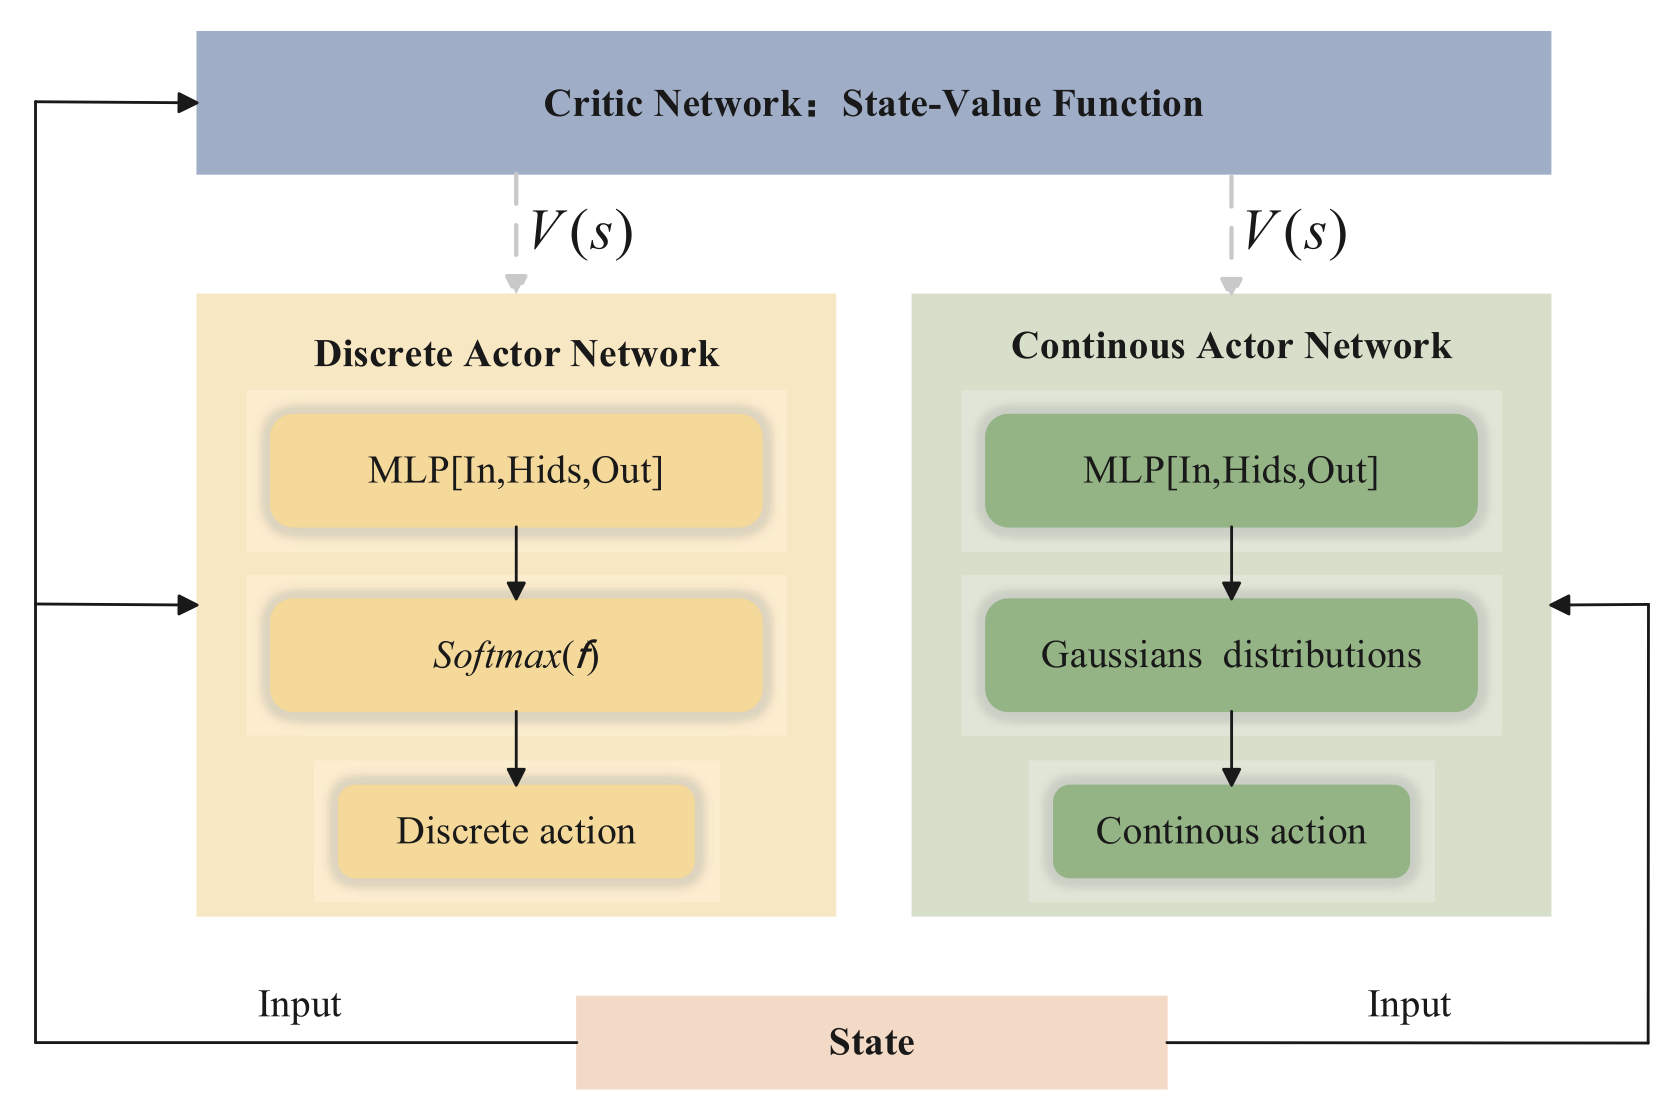
\includegraphics[width=\textwidth]{../images/pre_study/2ActorCriticNetworkArchitecture.png}
    \caption{Architecture of the proposed Actor-Critic Neural Network. Taken from (Zhao et al., 2026 \cite{ZHAO2026111784})}
    \label{fig:ac_architecture2}
\end{figure}
\textbf{Relevance and Comparative Analysis} \\
While the study by Zhao et al \cite{ZHAO2026111784}. addresses a more geographically complex passenger network, it provides a vital methodological benchmark for this thesis. Both approaches utilize action masking to enforce operational constraints; however, several key distinctions exist. While Zhao et al. \cite{ZHAO2026111784}  optimize for passenger flows using a hybrid HPPO actor-critic model, this thesis focuses on freight logistics ( specifically the transport of timber—within a two-line system ). 

Furthermore, instead of the dual-actor hybrid approach (HPPO) used in the cited study, this research employs a standard PPO algorithm with a single continuous actor. In this thesis, discrete requirements are handled by mapping continuous outputs to discrete values via a specialized mapping strategy, rather than maintaining a separate discrete actor network.


\section{Solving high-speed rolling stock planning with an improved LSTM-PPO reinforcement learning algorithm}
The work presented by Su et al. \cite{SU2026} investigates the Rolling Stock Planning (RSP) problem utilizing a PPO framework integrated with a Long Short-Term Memory (LSTM) network. To prevent the agent from converging on local optima, the authors incorporate a simulated annealing strategy, effectively balancing global exploration with local refinement. The choice of an LSTM architecture is specifically intended to capture temporal dependencies and provide the agent with a recursive memory of the episode's history. 

A fundamental assumption of this study is the prioritization of a fixed maintenance threshold over train departures, ensuring safety constraints are satisfied. The operational environment is modeled with three stations and a fixed scheduling regime, establishing a scenario closely aligned with the parameters of this thesis.

\textbf{State Space Representation} \\
The state at time step $t$ is defined by the history of assignments $V_t$ and the current task $x_t$. The history $V_t$ represents a comprehensive record of all train services already allocated to the $v$ rolling stock units (RSUs), while $x_t$ denotes the specific service currently awaiting assignment:
$$
V_t = \left\{ U_t^1 , U_t^2 , \ldots , U_t^v \right\} = \left\{ \left\{u_1^1 , u_2^1 , \ldots , u_r^1\right\} , \ldots , \left\{u_1^v , u_2^v , \ldots , u_r^v\right\} \right\}
$$

\textbf{Action Space Representation} \\
The agent is tasked with mapping the pending train service ($x_t$) to an available RSU ($v_i$). The resulting action is formulated as:
$$
a_t = (v_i, x_t)
$$
Consistent with the methodology adopted in this research, the action space is constrained by a filtering mechanism that automatically excludes actions violating operational requirements, such as maintenance schedules.

\textbf{Reward Mechanism} \\
The reward function is a multi-objective scalar derived from three primary components, each modulated by specific hyperparameters:
\begin{enumerate}
    \item $r_t^\text{connect}$: A positive reward for establishing a feasible connection between successive train services on the same RSU.
    \item $r_t^\text{save}$: An incentive aimed at minimizing the total number of RSUs required for operations.
    \item $r_t^\text{penalty}$: A penalty term for the violation of hard constraints, primarily regarding fixed maintenance intervals.
\end{enumerate}

\textbf{Relevance and Comparative Analysis} \\
The problem addressed by Su et al. \cite{SU2026} serves as a foundational benchmark for this thesis, although it represents a slightly simplified version of the real-world system as it focuses exclusively on RSU efficiency without considering passenger demand. 

There is a significant alignment between this thesis and Su et al. \cite{SU2026} regarding the prioritization of system safety; both models enforce maintenance requirements as a higher priority than schedule adherence. However, the maintenance modeling differs in flexibility: while  Su et al. \cite{SU2026} restricts maintenance to nighttime windows, this thesis allows the agent to execute early maintenance at any time to accommodate operational needs. Furthermore, while the present work omits dwell times as a deliberate simplification, this feature remains a viable candidate for future integration. Finally, although this thesis utilizes a Multi-Layer Perceptron (MLP) architecture rather than the LSTM employed by Su et al. \cite{SU2026}, the algorithmic structure of their work provided significant inspiration for the development of our proposed solution.
\begin{figure}[H]
    \centering
    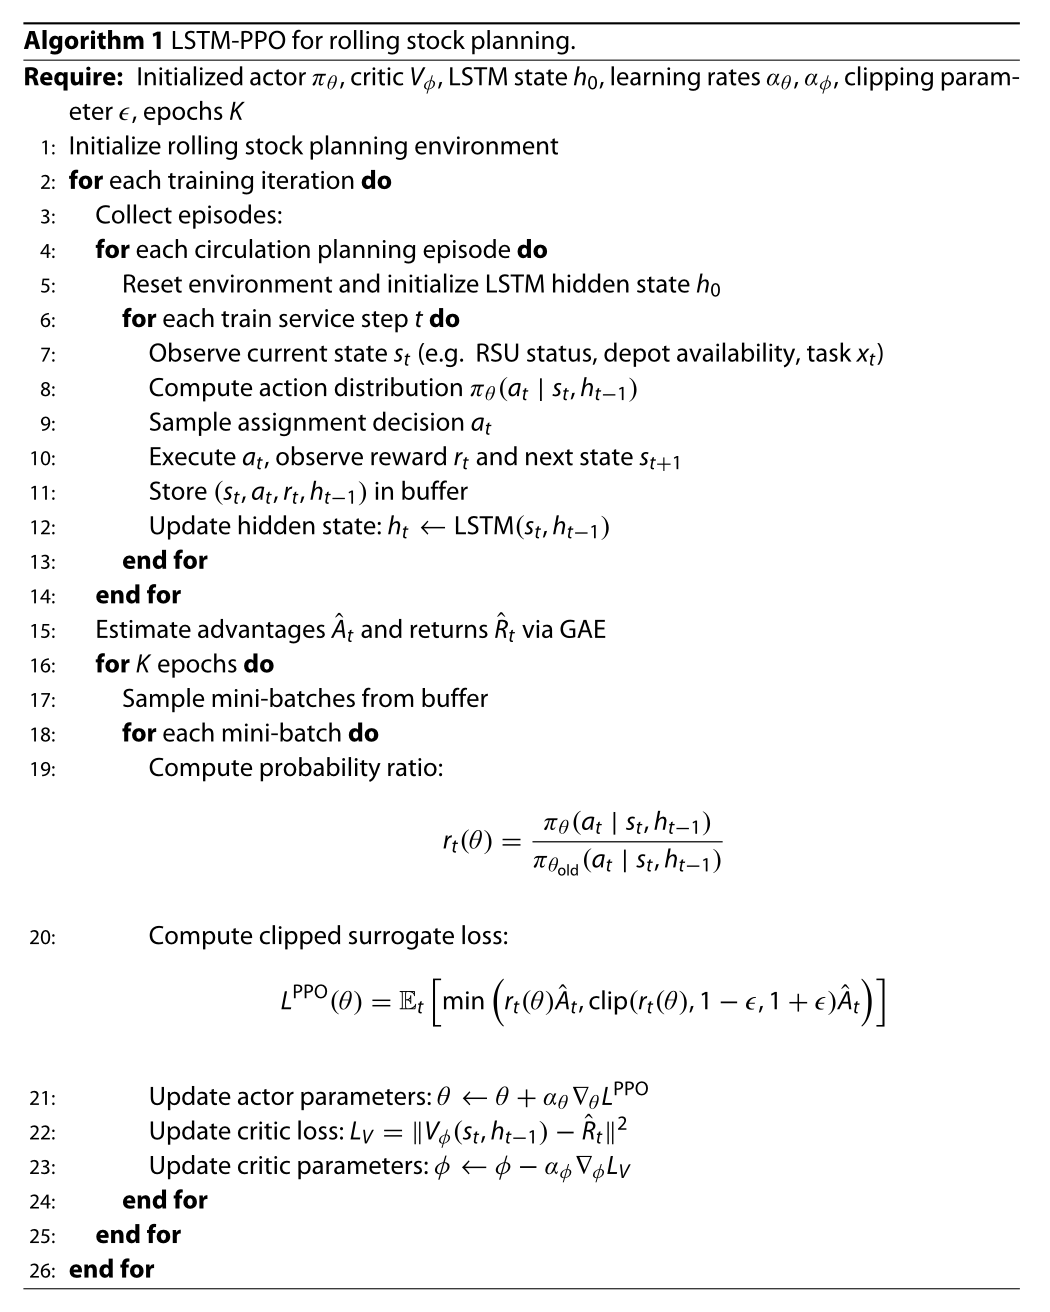
\includegraphics[width=\textwidth]{../images/pre_study/LSTM-PPO-Algorithm.png}
    \caption{PPO-LSTM Algorithm. Taken from (SU et al., 2026 \cite{SU2026}) }
    \label{fig:LSTM-PPO-Algorithm}
\end{figure}
% --- BIBLIOGRAPHY ---
\newpage
\bibliographystyle{plain} % This defines the style
\bibliography{references} % This looks for 'references.bib'
\end{document}